% DataSynth Executive Overview
% Compile with: pdflatex datasynth-executive-overview.tex (run twice for TOC + bibliography)
%               bibtex   datasynth-executive-overview
%               pdflatex datasynth-executive-overview.tex
%               pdflatex datasynth-executive-overview.tex
\documentclass[11pt,a4paper]{article}

% ── Packages ──────────────────────────────────────────────────────────────────
\usepackage[utf8]{inputenc}
\usepackage[T1]{fontenc}
\usepackage{lmodern}
\usepackage[margin=2.4cm]{geometry}
\usepackage{graphicx}
\usepackage{xcolor}
\usepackage{titlesec}
\usepackage{enumitem}
\usepackage{booktabs}
\usepackage{tabularx}
\usepackage{multirow}
\usepackage{fancyhdr}
\usepackage{hyperref}
\usepackage{tcolorbox}
\usepackage{needspace}
\usepackage{tikz}
\usepackage{pgfplots}
\usepackage{amssymb}
\usepackage[numbers]{natbib}
\pgfplotsset{compat=1.18}
\usetikzlibrary{arrows.meta, positioning, calc, shapes.geometric, backgrounds, fit}

% ── Single-source-of-truth version macros ────────────────────────────────────
\newcommand{\dsversion}{5.7.0}
\newcommand{\dsdate}{May 2026}
\newcommand{\dsrepourl}{https://github.com/mivertowski/SyntheticData}
\newcommand{\dsssrnurl}{https://ssrn.com/abstract=6538639}

% ── Colours ───────────────────────────────────────────────────────────────────
\definecolor{brand}{HTML}{1A2744}      % Deep navy
\definecolor{accent}{HTML}{2E86AB}     % Teal blue
\definecolor{highlight}{HTML}{F18F01}  % Amber
\definecolor{success}{HTML}{2D936C}    % Green
\definecolor{lightbg}{HTML}{F5F7FA}    % Light background
\definecolor{midgray}{HTML}{6C757D}    % Muted text

% ── Heading styles ────────────────────────────────────────────────────────────
\titleformat{\section}
  {\Large\bfseries\color{brand}}
  {\thesection}{1em}{}[\vspace{-0.4em}\textcolor{accent}{\rule{\textwidth}{1.2pt}}]

\titleformat{\subsection}
  {\large\bfseries\color{brand}}
  {\thesubsection}{0.8em}{}

\titleformat{\subsubsection}
  {\normalsize\bfseries\color{accent}}
  {\thesubsubsection}{0.6em}{}

% ── Header / Footer ──────────────────────────────────────────────────────────
\pagestyle{fancy}
\fancyhf{}
\renewcommand{\headrulewidth}{0.4pt}
\fancyhead[L]{\small\textcolor{midgray}{DataSynth --- Executive Overview}}
\fancyhead[R]{\small\textcolor{midgray}{v\dsversion}}
\fancyfoot[C]{\small\textcolor{midgray}{\thepage}}

% ── Custom boxes ──────────────────────────────────────────────────────────────
\tcbset{
  keybox/.style={
    colback=lightbg, colframe=accent, boxrule=0.6pt,
    arc=3pt, left=8pt, right=8pt, top=6pt, bottom=6pt,
    fonttitle=\bfseries\color{brand}, title=#1
  },
  statbox/.style={
    colback=white, colframe=brand, boxrule=0.8pt,
    arc=4pt, left=6pt, right=6pt, top=4pt, bottom=4pt,
    width=0.30\textwidth
  },
  notebox/.style={
    colback=lightbg!60, colframe=midgray, boxrule=0.4pt,
    arc=2pt, left=8pt, right=8pt, top=4pt, bottom=4pt,
    fonttitle=\bfseries\small\color{brand}, title=#1
  }
}

% ── Hyperref setup ────────────────────────────────────────────────────────────
\hypersetup{
  colorlinks=true,
  linkcolor=brand,
  urlcolor=accent,
  citecolor=accent,
  pdftitle={DataSynth -- Enterprise Synthetic Data Platform},
  pdfauthor={Michael Ivertowski},
  pdfsubject={Executive Overview, v\dsversion},
}

% ══════════════════════════════════════════════════════════════════════════════
\begin{document}

% ── Title page ────────────────────────────────────────────────────────────────
\begin{titlepage}
\begin{tikzpicture}[remember picture, overlay]
  \fill[brand] (current page.north west) rectangle
    ([yshift=-9cm]current page.north east);
  \fill[accent] ([yshift=-9cm]current page.north west) rectangle
    ([yshift=-9.4cm]current page.north east);
  \foreach \x in {0.5,1.0,...,5.0} {
    \foreach \y in {0.5,1.0,...,3.0} {
      \fill[white, opacity=0.04] ([xshift=\x cm, yshift=-\y cm]current page.north west)
        circle (1.5pt);
    }
  }
\end{tikzpicture}

\vspace*{1.5cm}
\begin{flushleft}
  {\fontsize{38}{44}\selectfont\bfseries\textcolor{white}{DataSynth}}\\[0.5em]
  {\fontsize{16}{20}\selectfont\textcolor{white!85}{Enterprise Synthetic Data Platform}}\\[0.3em]
  {\large\textcolor{white!65}{Reference Knowledge Graphs for Audit Analytics \& ML}}\\[0.3em]
  {\normalsize\textcolor{white!50}{Rust core \textbullet{} 17 modular crates \textbullet{}
    Group Audit Engine \textbullet{} Audit-Methodology Layer}}
\end{flushleft}

\vspace{5.5cm}

\begin{flushleft}
  \textcolor{midgray}{\large Executive Overview}\\[0.8em]
  {\Large\textcolor{brand}{\textbf{Version \dsversion}}}\\[1.5em]
  \textcolor{midgray}{%
    Deterministic, privacy-preserving synthetic data generation\\
    for enterprise finance, group audit, compliance testing,\\
    and machine learning.%
  }
\end{flushleft}

\vfill
\begin{flushleft}
  \textcolor{midgray}{\small
    \textbf{Companion paper:} Ivertowski, M. (2026).
    \textit{DataSynth: Reference Knowledge Graphs for Enterprise Audit Analytics
    through Synthetic Data Generation with Provable Statistical Properties.}\\
    SSRN: \href{\dsssrnurl}{ssrn.com/abstract=6538639}
    \textbullet{} In-repo: \texttt{paper/main.tex}\\[6pt]
    Built with Rust \textbullet{} 17 active crates \textbullet{} 200\,K+ entries/sec\\[4pt]
    Open-source (Apache-2.0) \textbullet{} Commercial SDKs at
    \href{https://vynfi.com}{vynfi.com}\\[4pt]
    \textbf{GitHub:} \url{\dsrepourl}
  }
\end{flushleft}
\end{titlepage}

% ── Table of Contents ─────────────────────────────────────────────────────────
\tableofcontents
\newpage

% ══════════════════════════════════════════════════════════════════════════════
\section{Executive Summary}

DataSynth is a high-performance synthetic data platform purpose-built for
enterprise accounting, group audit, audit analytics, and machine learning.
Written in Rust for maximum throughput and memory safety, it generates
realistic, internally coherent financial data that satisfies the statistical
and structural properties of real-world enterprise resource planning (ERP)
systems --- and, since v5.0, an entire \emph{multi-entity group consolidation}
on top, IFRS / IAS 21 / IAS 28 / IFRS 10 compliant by construction.

\begin{tcolorbox}[keybox={Three pillars}]
\begin{itemize}[leftmargin=1.2em, itemsep=4pt]
  \item \textbf{Enterprise simulation depth} --- 14 process families (GL, P2P,
        O2C, S2C, H2R, manufacturing, financial reporting, tax, treasury,
        ESG, banking/AML, audit, intercompany, period close), 100+ output
        tables, generation-time invariants (debits = credits,
        Assets = Liabilities + Equity, Benford compliance).
  \item \textbf{Multi-entity group audit} --- a three-phase manifest /
        shard / aggregate engine produces standalone single-entity archives
        \emph{plus} consolidated FS, IC matching, eliminations, IAS 21
        translation, NCI / equity-method rollforwards, CGU goodwill
        impairment testing, and chained multi-period continuity.
  \item \textbf{Methodology-driven audit trail} --- the
        \texttt{datasynth-audit-fsm} crate ships a typed audit-methodology
        layer: Big-4 ISA spine (4 phases, 17 procedures), 4 firm overlays,
        7 jurisdictional overlays, 6 KYC/AML workflows, banking-form
        ontologies, Bayesian RMM scoring, an L4 typed property-graph
        schema, and SHA-256 Merkle tamper-evidence for working-paper
        bundles.
\end{itemize}
\end{tcolorbox}

\begin{tcolorbox}[keybox={Why DataSynth?}]
\begin{itemize}[leftmargin=1.2em, itemsep=3pt]
  \item \textbf{No real data required} --- eliminates privacy, regulatory, and
        procurement barriers to analytics development.
  \item \textbf{Full auditability} --- deterministic, seeded generation;
        every dataset is bit-for-bit reproducible.
  \item \textbf{ML-ready from day one} --- ground-truth labels for fraud,
        anomalies, data quality issues, and ISA-240 audit flags ship
        alongside every record.
  \item \textbf{Domain depth} --- the full accounting lifecycle, multi-entity
        consolidation, and complete audit methodology.
  \item \textbf{Empirically grounded} --- statistical distributions calibrated
        against real enterprise data; formal proofs in the companion paper
        \citep{ivertowski2026datasynth}.
  \item \textbf{Provenance you can verify} --- per-file SHA-256, W3C PROV-JSON
        lineage graphs, and Merkle-rooted working-paper bundles.
\end{itemize}
\end{tcolorbox}

\subsection{At a Glance}

\vspace{0.6em}
\begin{center}
\begin{tabular}{@{}c@{\hspace{1.8em}}c@{\hspace{1.8em}}c@{}}
\begin{tcolorbox}[statbox, width=4.8cm]
  \centering
  {\fontsize{26}{30}\selectfont\bfseries\textcolor{accent}{200\,K+}}\\[3pt]
  {\small entries/sec (single thread)}
\end{tcolorbox} &
\begin{tcolorbox}[statbox, width=4.8cm]
  \centering
  {\fontsize{26}{30}\selectfont\bfseries\textcolor{accent}{17}}\\[3pt]
  {\small modular Rust crates}
\end{tcolorbox} &
\begin{tcolorbox}[statbox, width=4.8cm]
  \centering
  {\fontsize{26}{30}\selectfont\bfseries\textcolor{accent}{14}}\\[3pt]
  {\small enterprise process families}
\end{tcolorbox} \\[0.8em]
\begin{tcolorbox}[statbox, width=4.8cm]
  \centering
  {\fontsize{26}{30}\selectfont\bfseries\textcolor{accent}{12+7}}\\[3pt]
  {\small Big-4 + jurisdictional audit overlays}
\end{tcolorbox} &
\begin{tcolorbox}[statbox, width=4.8cm]
  \centering
  {\fontsize{26}{30}\selectfont\bfseries\textcolor{accent}{8}}\\[3pt]
  {\small IFRS / IAS standards modelled}
\end{tcolorbox} &
\begin{tcolorbox}[statbox, width=4.8cm]
  \centering
  {\fontsize{26}{30}\selectfont\bfseries\textcolor{accent}{60+}}\\[3pt]
  {\small ACFE-aligned fraud schemes}
\end{tcolorbox} \\[0.8em]
\begin{tcolorbox}[statbox, width=4.8cm]
  \centering
  {\fontsize{26}{30}\selectfont\bfseries\textcolor{accent}{6}}\\[3pt]
  {\small KYC / AML workflows}
\end{tcolorbox} &
\begin{tcolorbox}[statbox, width=4.8cm]
  \centering
  {\fontsize{26}{30}\selectfont\bfseries\textcolor{accent}{4}}\\[3pt]
  {\small differential-privacy levels}
\end{tcolorbox} &
\begin{tcolorbox}[statbox, width=4.8cm]
  \centering
  {\fontsize{26}{30}\selectfont\bfseries\textcolor{accent}{100+}}\\[3pt]
  {\small output tables (CSV / JSON / Parquet / XBRL)}
\end{tcolorbox} \\[0.8em]
\begin{tcolorbox}[statbox, width=4.8cm]
  \centering
  {\fontsize{26}{30}\selectfont\bfseries\textcolor{accent}{5}}\\[3pt]
  {\small industry presets}
\end{tcolorbox} &
\begin{tcolorbox}[statbox, width=4.8cm]
  \centering
  {\fontsize{26}{30}\selectfont\bfseries\textcolor{accent}{15}}\\[3pt]
  {\small holiday calendar regions}
\end{tcolorbox} &
\begin{tcolorbox}[statbox, width=4.8cm]
  \centering
  {\fontsize{26}{30}\selectfont\bfseries\textcolor{accent}{XBRL}}\\[3pt]
  {\small 2.1 instance export (US GAAP \& IFRS)}
\end{tcolorbox}
\end{tabular}
\end{center}

\begin{tcolorbox}[notebox={Companion paper}]
Formal statements of the distributional, copula, and DP-composition
properties summarised in this overview --- together with proofs and
ablation studies --- appear in the companion paper
\citep{ivertowski2026datasynth}. Readers building academic benchmarks or
formal evaluations should consult \S\S 5--9 of the paper directly. The
LaTeX source is available in-repo at \texttt{paper/main.tex}.
\end{tcolorbox}

% ══════════════════════════════════════════════════════════════════════════════
\newpage
\section{Reference Knowledge Graphs}

DataSynth builds what the companion paper calls a \emph{reference knowledge
graph}: a deterministic, content-addressable graph whose nodes encode every
domain entity (companies, vendors, customers, accounts, journal entries,
controls, procedures, evidence) and whose edges encode every business
relationship (transactions, references, ownership, control coverage,
assertion linkage, evidence support). Generation is reproducible byte-for-byte
from a seed, so the same graph can be regenerated, hashed, signed, and
audited.

\subsection{The L4 Audit-Graph Schema}

The audit-methodology layer ships a \textbf{typed property-graph schema} ---
11 node types crossed with 10 edge types --- that mirrors the assertion-
and risk-driven structure of an ISA / PCAOB engagement.

\begin{center}
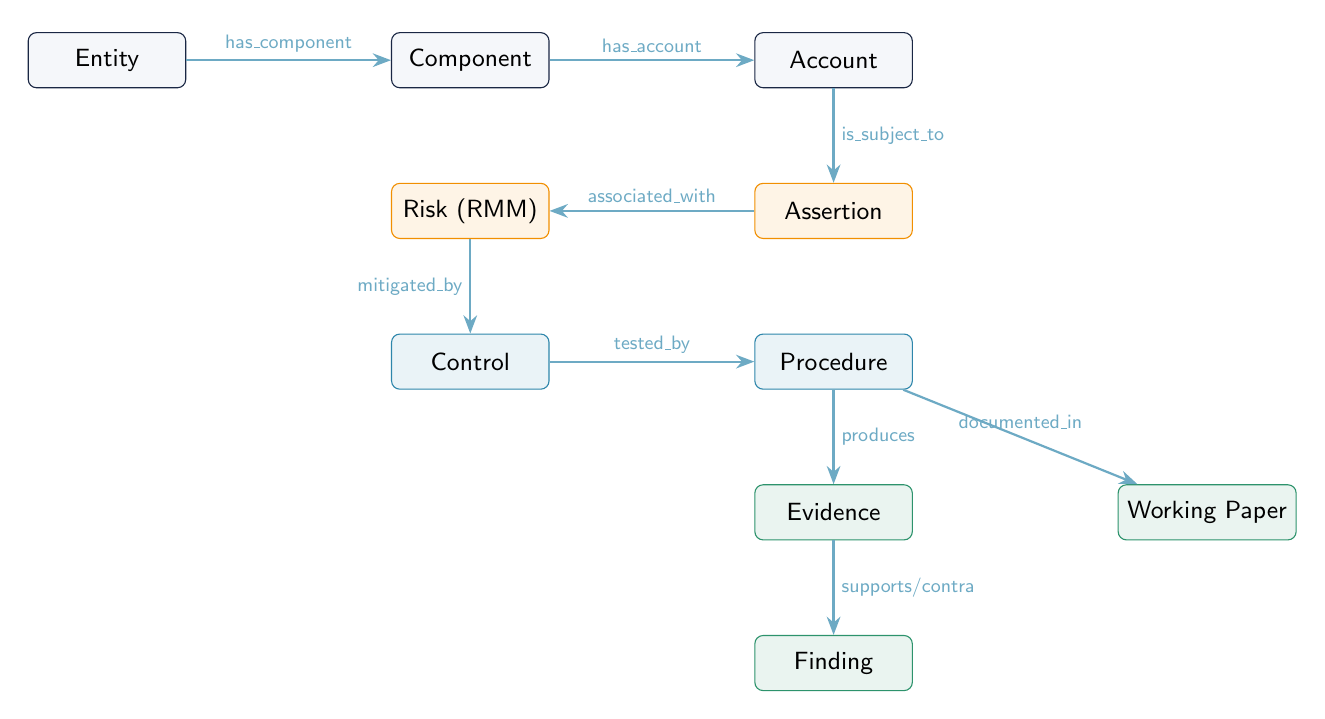
\begin{tikzpicture}[
  >=Stealth,
  node distance=1.6cm and 2.6cm,
  every node/.style={font=\small\sffamily},
  ent/.style={draw=brand, fill=lightbg, rounded corners=3pt,
              minimum width=2.0cm, minimum height=0.7cm, align=center},
  risk/.style={draw=highlight, fill=highlight!10, rounded corners=3pt,
               minimum width=2.0cm, minimum height=0.7cm, align=center},
  proc/.style={draw=accent, fill=accent!10, rounded corners=3pt,
               minimum width=2.0cm, minimum height=0.7cm, align=center},
  evid/.style={draw=success, fill=success!10, rounded corners=3pt,
               minimum width=2.0cm, minimum height=0.7cm, align=center},
  edge/.style={->, thick, color=accent!70}
]
  \node[ent] (entity)    {Entity};
  \node[ent, right=of entity] (component) {Component};
  \node[ent, right=of component] (account)  {Account};
  \node[risk, below=1.2cm of account] (assertion) {Assertion};
  \node[risk, left=2.6cm of assertion] (risk) {Risk (RMM)};
  \node[proc, below=1.2cm of risk] (control) {Control};
  \node[proc, right=of control] (procedure) {Procedure};
  \node[evid, below=1.2cm of procedure] (evidence) {Evidence};
  \node[evid, right=of evidence] (wp) {Working Paper};
  \node[evid, below=1.2cm of evidence] (finding) {Finding};

  \draw[edge] (entity)    -- node[above,midway,scale=0.78]{has\_component} (component);
  \draw[edge] (component) -- node[above,midway,scale=0.78]{has\_account}   (account);
  \draw[edge] (account)   -- node[right,midway,scale=0.78]{is\_subject\_to} (assertion);
  \draw[edge] (assertion) -- node[above,midway,scale=0.78]{associated\_with} (risk);
  \draw[edge] (risk)      -- node[left,midway,scale=0.78]{mitigated\_by}    (control);
  \draw[edge] (control)   -- node[above,midway,scale=0.78]{tested\_by}     (procedure);
  \draw[edge] (procedure) -- node[right,midway,scale=0.78]{produces}       (evidence);
  \draw[edge] (procedure) -- node[above,midway,scale=0.78]{documented\_in} (wp);
  \draw[edge] (evidence)  -- node[right,midway,scale=0.78]{supports/contra} (finding);
\end{tikzpicture}
\end{center}

This schema is the same one a Big-4 firm carries in its proprietary
audit-management software --- only here it is open, content-addressable, and
generated end-to-end alongside the underlying ledger. The companion paper
formalises it as a typed property graph and proves the soundness of the
acceptance-gate predicates that consume it.

\subsection{Why Knowledge Graphs}

A reference graph turns the audit dataset from a collection of CSVs into a
\textbf{queryable, verifiable, and benchmarkable artefact}:

\begin{itemize}[leftmargin=1.2em, itemsep=3pt]
  \item Cross-process queries (vendor $\to$ PO $\to$ GR $\to$ invoice $\to$
        payment $\to$ JE $\to$ control $\to$ procedure $\to$ working paper)
        are graph traversals, not multi-table SQL joins.
  \item Provenance is intrinsic --- every node carries its generator type,
        seed, and generation timestamp; every edge carries its derivation
        rule.
  \item Anomalies travel through the graph: when a fraudulent vendor
        invoice is injected, the propagation path through document flows,
        JE postings, and control failures is observable.
  \item ML benchmarks become reproducible --- the same seed yields the
        same graph, so model A and model B can be compared on the
        \emph{exact} same data without re-randomisation.
\end{itemize}

% ══════════════════════════════════════════════════════════════════════════════
\newpage
\section{Enterprise Process Simulation}

Every process chain produces cross-referenced master data, documents, and
journal entries that respect double-entry bookkeeping, document chain
integrity, and balance sheet equation invariants \emph{at generation time}.

\subsection{Process Families}

\renewcommand{\arraystretch}{1.25}
\begin{tabularx}{\textwidth}{@{}>{\bfseries\color{brand}}l X@{}}
\toprule
\textbf{Process family} & \textbf{Scope} \\
\midrule
General Ledger      & Journal entries, chart of accounts (small / medium / large), ACDOCA, balanced postings, FX revaluation \\
Procure-to-Pay      & POs, goods receipts, vendor invoices, payments, three-way match with configurable tolerances \\
Order-to-Cash       & Sales orders, deliveries, customer invoices, receipts, dunning, AR aging \\
Source-to-Contract  & Spend analysis, sourcing projects, supplier qualification, RFx, bids, contracts, scorecards \\
Hire-to-Retire      & Payroll, time \& attendance, expenses, benefits, defined-benefit pensions, stock-based compensation \\
Manufacturing       & Production orders, BOMs, WIP costing, quality inspections, cycle counts, inventory movements \\
Financial Reporting & BS / IS / CF, statement of changes in equity, KPIs, budgets, segment reporting, notes, XBRL \\
Tax                 & Multi-jurisdiction VAT / GST, ASC 740 / IAS 12 provisions, deferred tax rollforward, withholding tax, uncertain tax positions \\
Treasury            & Cash positioning, forecasts, pooling, hedging (ASC 815 / IFRS 9), debt covenants, derivatives \\
ESG                 & GHG Scope 1/2/3, energy / water / waste, workforce diversity, pay equity, GRI / SASB / TCFD disclosures \\
Banking / AML       & 20 AML typologies, criminal networks, velocity features, KYC tiers, SAR narratives \\
Audit               & ISA lifecycle, ISA 600 group audit, SOX 302/404, methodology blueprints \\
Intercompany        & IC matching (multi-strategy), transfer pricing methods, eliminations, currency translation, NCI \\
Period Close        & Depreciation runs, accruals, year-end closing, tax provisions, FX revaluation \\
\bottomrule
\end{tabularx}

\subsection{Coherence Engine}

A cross-module coherence layer connects every record to every other record:

\begin{itemize}[leftmargin=1.2em, itemsep=3pt]
  \item \textbf{Document chains} --- PO\,$\to$\,GR\,$\to$\,Invoice\,$\to$\,Payment
        with proper reference fields and audit-trail flags.
  \item \textbf{Vendor/customer networks} --- 3-tier supply chain (Tier1 / 2 / 3),
        4 cluster types (reliable strategic / standard / transactional / problematic),
        configurable concentration risk, and bilateral relationships.
  \item \textbf{Customer segmentation} --- 4 value segments with prescribed
        revenue/customer share, lifecycle stages, referral networks, corporate
        hierarchies.
  \item \textbf{Relationship strength} --- weighted composite of transaction
        volume (log scale), count (sqrt scale), duration, recency
        (90-day exponential decay), and mutual connections (Jaccard index).
  \item \textbf{Cross-process links} --- inventory $\leftrightarrow$ P2P/O2C,
        payment $\leftrightarrow$ bank reconciliation, intercompany bilateral
        matching.
\end{itemize}

\subsection{Standards Coverage (Single Entity)}

Single-entity output adheres to the following standards by construction:

\renewcommand{\arraystretch}{1.2}
\begin{tabularx}{\textwidth}{@{}>{\bfseries\color{brand}}l X@{}}
\toprule
\textbf{Domain} & \textbf{Standard \& artefacts} \\
\midrule
Revenue                       & ASC 606 / IFRS 15: customer contracts, performance obligations, revenue allocation, contract modifications \\
Leases                        & ASC 842 / IFRS 16: ROU assets, lease liabilities, finance / operating split \\
Fair Value                    & ASC 820 / IFRS 13: Level 1/2/3 hierarchy, valuation methodology disclosures \\
Impairment                    & ASC 360 / IAS 36: triggering events, recoverable-amount tests, no-reversal rule \\
Business Combinations         & IFRS 3 / ASC 805: PPA, goodwill, fair-value adjustments, contingent consideration, bargain purchase \\
ECL Provisions                & IFRS 9: 12-month / lifetime ECL stages, provision matrix, ECL movements \\
Provisions                    & IAS 37 / ASC 450: provision liabilities, contingent liabilities, unwind of discount \\
Pensions                      & IAS 19 / ASC 715: defined-benefit obligation, plan assets, OCI remeasurements \\
Stock Compensation            & ASC 718: grant-date fair value, vesting, APIC stock-comp \\
Internal Controls (SOX)       & SOX 302 certifications, SOX 404 assessments, deficiency matrix, material-weakness classification \\
ISA Audit Lifecycle           & 34 ISA standards mapped, analytical procedures (ISA 520), confirmations (ISA 505), opinions (ISA 700/705/706/701) \\
Audit Data Exchange           & ISO 21378:2019 (Audit Data Collection): 3-level account classification (Type / Class / Sub-Class) populated on every CoA account and every JE row, with descriptive names alongside the ISO codes \\
Industry Account Packs        & v5.7.0: opt-in 6-digit sub-account expansion driven by sector-specific YAML packs (manufacturing / retail / financial services / healthcare / technology); deterministic-by-document picker for stable sub-account selection \\
\bottomrule
\end{tabularx}

% ══════════════════════════════════════════════════════════════════════════════
\newpage
\section{Group Audit Engine}

Since v5.0, DataSynth ships a \textbf{multi-entity group audit engine}
layered above the single-entity pipeline. Per-entity generation stays
byte-identical to the standalone flow; the consolidation logic lives entirely
in the \texttt{datasynth-group} crate. The pipeline is a deterministic
\textbf{three-phase model}.

\subsection{Three-Phase Architecture}

\vspace{0.4em}
\begin{center}
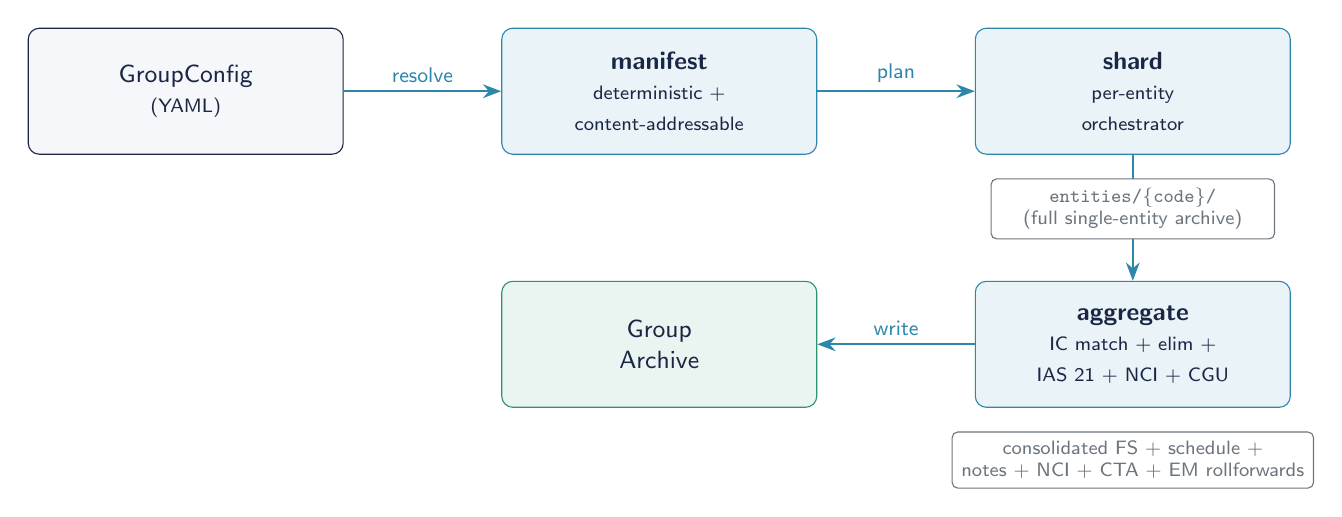
\begin{tikzpicture}[
  >=Stealth,
  every node/.style={font=\small\sffamily},
  phase/.style={draw=brand, fill=lightbg, rounded corners=4pt,
                minimum width=4.0cm, minimum height=1.6cm, align=center,
                text=brand},
  artefact/.style={draw=midgray, fill=white, rounded corners=2pt,
                   minimum width=3.6cm, minimum height=0.7cm, align=center,
                   text=midgray, font=\scriptsize\sffamily},
  edge/.style={->, thick, color=accent}
]
  \node[phase] (config) {GroupConfig\\{\scriptsize (YAML)}};
  \node[phase, right=2.0cm of config, fill=accent!10, draw=accent] (manifest)
    {\textbf{manifest}\\{\scriptsize deterministic +}\\{\scriptsize content-addressable}};
  \node[phase, right=2.0cm of manifest, fill=accent!10, draw=accent] (shard)
    {\textbf{shard}\\{\scriptsize per-entity}\\{\scriptsize orchestrator}};
  \node[phase, below=1.6cm of shard, fill=accent!10, draw=accent] (aggregate)
    {\textbf{aggregate}\\{\scriptsize IC match + elim +}\\{\scriptsize IAS 21 + NCI + CGU}};
  \node[phase, left=2.0cm of aggregate, fill=success!10, draw=success] (output)
    {Group\\Archive};

  \draw[edge] (config)   -- node[above,midway,scale=0.85]{resolve} (manifest);
  \draw[edge] (manifest) -- node[above,midway,scale=0.85]{plan}    (shard);
  \draw[edge] (shard)    -- node[right,midway,scale=0.85]{entity TBs} (aggregate);
  \draw[edge] (aggregate) -- node[above,midway,scale=0.85]{write} (output);

  % Per-entity archives note
  \node[artefact, below=0.3cm of shard, xshift=0cm] (sharddetail)
    {\texttt{entities/\{code\}/}\\(full single-entity archive)};

  % Aggregate outputs note
  \node[artefact, below=0.3cm of aggregate] (aggdetail)
    {consolidated FS + schedule +\\notes + NCI + CTA + EM rollforwards};
\end{tikzpicture}
\end{center}

\begin{enumerate}[leftmargin=1.4em, itemsep=4pt]
  \item \textbf{\texttt{manifest}} resolves a \texttt{GroupConfig} into a
        deterministic, content-addressable \texttt{GroupManifest} ---
        entities, periods, ownership graph, IC pair plan, shard plan,
        FX / chart-of-accounts masters, audit engagement plan, tax group plan.
  \item \textbf{\texttt{shard}} drives the orchestrator for one shard of
        entities and writes a full single-entity archive per entity under
        \texttt{entities/\{code\}/}.
  \item \textbf{\texttt{aggregate}} reads shard outputs and runs IC matching,
        eliminations, IAS 21 currency translation, NCI rollforward,
        equity-method investments (with suppressed-loss tracking), CGU
        goodwill-impairment testing, and writes consolidated FS, schedule,
        notes, and rollforwards.
\end{enumerate}

The CLI auto-detects whether an input config is a \texttt{GroupConfig} (top-
level \texttt{presentation\_currency} + \texttt{ownership} keys) and dispatches
to the group pipeline transparently --- existing single-entity configs continue
to work unchanged.

\subsection{Standards Coverage (Group)}

\renewcommand{\arraystretch}{1.2}
\begin{tabularx}{\textwidth}{@{}>{\bfseries\color{brand}}l X@{}}
\toprule
\textbf{Standard} & \textbf{What is modelled} \\
\midrule
IAS 21 \S{}39 / \S{}42(b) & Closing-rate translation, CTA rollforward; closing-rate-for-all-items in hyperinflationary economies \\
IAS 28 \S{}22 / \S{}38    & Equity-method investments; suppressed-loss tracking with recovery-against-future-profits \\
IAS 29 \S{}12             & Indexed restatement before IAS 21 closing-rate translation \\
IAS 36 \S{}10 / 80 / 104 / 124 & CGU definition, acquisition-date goodwill allocation, impairment-loss allocation, no-reversal rule \\
IFRS 3 \S{}19 / \S{}42    & Acquisition-date NCI measurement (full vs partial goodwill); mid-period ControlGained re-measurement at fair value \\
IFRS 5 / ASC 810          & NCI presented separately from controlling-interest equity \\
IFRS 8.13 / ASC 280-10-50-41 & Operating-segment disclosures derived from the ownership graph \\
IFRS 10.23 / IFRS 10.B97  & Equity-transaction adjustment for within-control ownership changes; deconsolidation on control loss \\
\bottomrule
\end{tabularx}

\subsection{Multi-Period Continuity}

The \texttt{group generate-chain} subcommand stitches engagements together
across periods. Opening balances, NCI, CTA, and equity-method carryforwards
flow forward without caller plumbing; the chain helpers handle
emergent-fuzzy IC matching tolerances, mid-period acquisitions and
disposals, and step-acquisition mid-period control-gained transitions
(IFRS 3 \S{}42 P\&L re-measurement and time-weighted profit attribution).

\subsection{Output Layout}

\begin{tcolorbox}[notebox={Per-engagement archive}]
\small
\begin{verbatim}
./group_archive/
  manifest.json                          # canonical group manifest
  entities/
    NESTLE_SA/      (full single-entity archive per shard)
    NESTLE_USA/     ...
  consolidated/
    consolidated_financial_statements.json
    consolidation_schedule.json
    notes_to_consolidated_fs.json
    nci_rollforward.json
    cta_rollforward.json
    translation_worksheet.json
    equity_method_investments.json
    equity_method_suppressed_losses.json
    cgu_impairment_tests.json
  ic_eliminations/ic_matching_coverage.json
  shard_summary.json
\end{verbatim}
\end{tcolorbox}

% ══════════════════════════════════════════════════════════════════════════════
\newpage
\section{Audit-Methodology Layer}

The \texttt{datasynth-audit-fsm} crate (v5.5.0) ships a typed
audit-methodology layer derived from the
\href{https://github.com/mivertowski/AuditMethodology}{AuditMethodology}
companion repository. All blueprints, overlays, ontologies, and form
schemas are embedded via \texttt{include\_str!} so loaders are zero-I/O at
runtime. The L4 graph schema introduced in \S{}2 is the integration surface.

\subsection{What Ships in the Layer}

\renewcommand{\arraystretch}{1.25}
\begin{tabularx}{\textwidth}{@{}>{\bfseries\color{brand}}l X@{}}
\toprule
\textbf{Module} & \textbf{What it carries} \\
\midrule
\texttt{big4\_methodology} &
  ISA-derived common spine (4 phases, 17 procedures) plus 4 firm overlays
  inheriting from the spine (EY GAM, PwC Aura, KPMG Clara, Deloitte Omnia)
  with per-procedure firm tools and signoff chains, plus a cross-firm
  equivalence map for harmonisation reporting. \\
\texttt{jurisdictional\_overlay} &
  7 overlays --- PCAOB, EU CSRD, UK FRC, ASIC (Australia), JFSA (Japan),
  ACRA (Singapore), HKICPA (Hong Kong) --- 39 procedures total, AND-logic
  resolution on \texttt{(jurisdiction $\times$ registrant\_type)}. \\
\texttt{methodology\_blueprint} &
  ISA 600 (Revised, December 2022) and CSRD limited-assurance methodology
  blueprints. \\
\texttt{kyc\_blueprint} &
  6 KYC / AML workflows --- private banking, correspondent banking,
  crypto-CASP, periodic KYC, SAR escalation, sanctions-hit remediation. \\
\texttt{banking\_forms} &
  7 banking form ontologies (MROS SAR, 4 UBS forms, Wolfsberg CBDDQ, FCCQ)
  and a 228-entry cross-form evidence index unifying fields under canonical
  terms. \\
\texttt{scenario\_library} &
  15 deterministic engagement scenarios with expected outcomes (opinion
  type, going-concern conclusion, EOM paragraph, acceptance gate) for
  FSM verification. \\
\texttt{rmm\_scoring} &
  Bayesian Risk-of-Material-Misstatement scoring --- 12-factor taxonomy
  (7 inherent + 5 control), conjugate Beta-Bernoulli updates,
  RMM = IR $\times$ CR aggregation. \\
\texttt{l4\_graph} &
  Typed property-graph schema, 11 node types $\times$ 10 edge types
  (see \S{}2). \\
\texttt{working\_paper\_merkle} &
  SHA-256 Merkle tree with replay-protected inclusion proofs;
  ISA 230 working-paper / engagement-bundle types; canonical
  \texttt{bundle\_root} ordered by \texttt{wp\_id}. \\
\bottomrule
\end{tabularx}

\subsection{Legacy YAML-Driven FSM (Still Available)}

The earlier YAML-driven FSM engine (10 built-in blueprints --- FSA, IA, KPMG,
PwC, Deloitte, EY GAM, SOC 2, PCAOB, Regulatory) remains available alongside
the new modules. Existing integrations continue to work unchanged; new work
is recommended on the typed audit-methodology layer for type safety,
zero-I/O startup, and Merkle tamper-evidence.

\subsection{Output Artefacts}

For each engagement the audit generators produce: engagement letters,
combined risk assessments (ISA 315), materiality calculations (ISA 320),
sampling plans + sampled items (ISA 530), accounting estimates (ISA 540),
analytical procedures (ISA 520), confirmations (ISA 505), going-concern
assessments (ISA 570), subsequent events (ISA 560), service-organization
SOC reports (ISA 402), component-auditor reports (ISA 600),
audit opinions + key audit matters (ISA 700/705/706/701),
SOX 302 / 404 documentation, ISA / PCAOB cross-reference mappings, and
SHA-256 Merkle bundle roots.

% ══════════════════════════════════════════════════════════════════════════════
\newpage
\section{Statistical Foundations}

DataSynth amounts, frequencies, correlations, and temporal patterns follow
empirical distributions calibrated against real enterprise data. This section
sketches the model; \textbf{formal statements and proofs appear in the
companion paper, \S\S{}5--9} \citep{ivertowski2026datasynth}.

\subsection{Distributions in the Pipeline}

\renewcommand{\arraystretch}{1.2}
\begin{tabularx}{\textwidth}{@{}>{\bfseries\color{brand}}l X@{}}
\toprule
\textbf{Family} & \textbf{Use} \\
\midrule
Log-normal mixtures      & Amount sampling --- routine / significant / major components with weighted mixing \\
Benford's Law            & First-digit law compliance with measurable MAD; supports first-digit, first-two-digit, and deviation-injection variants \\
Gaussian copulas         & Cross-field dependency modelling (amount $\times$ line items $\times$ approval level) with rank-preserving inverse-CDF sampling \\
Clayton / Gumbel / Frank / Student-t & Tail-asymmetric dependence; lower-tail (Clayton) for fraud co-incidence, upper-tail (Gumbel) for shared peak loads \\
Pareto                   & Heavy-tailed amounts (vendor concentration, customer revenue) \\
Weibull                  & Time-to-event modelling (payment delays, dunning escalation) \\
Beta                     & Proportions and percentages (tax rates, allocation ratios) \\
Zero-inflated            & Cost centres, line items where many records carry no value \\
Conditional              & Breakpoint-based generation: amount conditional on document type, vendor tier, etc. \\
Drift / regime change    & Economic cycles, recession depth, growth phases over multi-year horizons \\
Temporal                 & Seasonality, holiday calendars (15 regions), business-day conventions, T+N settlement, period-end clustering \\
\bottomrule
\end{tabularx}

\subsection{Validation Tests (Always-On)}

\begin{itemize}[leftmargin=1.2em, itemsep=3pt]
  \item \textbf{Benford first-digit MAD} --- threshold 0.015 (significant
        deviation by Nigrini's classification).
  \item \textbf{Distribution fit} --- Anderson-Darling and chi-squared
        against the configured target, $\alpha = 0.05$.
  \item \textbf{Correlation check} --- Spearman rank correlation against
        the configured copula, $\alpha = 0.05$.
  \item \textbf{Balance equation} --- assets $=$ liabilities $+$ equity,
        every JE balanced, every period.
\end{itemize}

\subsection{Industry Profiles}

Five built-in industry profiles --- Retail, Manufacturing, Financial Services,
Healthcare, Technology --- pre-configure distributions, vendor counts,
customer segmentation, fraud rates, and process emphasis. Three complexity
tiers (Small / Medium / Large) drive chart-of-accounts sizing and
transaction volume.

% ══════════════════════════════════════════════════════════════════════════════
\newpage
\section{AI-Augmented Generation}

\subsection{Neural Diffusion}

A Candle-powered score network (DDPM) trained end-to-end on tabular feature
slices, with deterministic sampling. GPU acceleration via the
\texttt{neural-cuda} feature flag with a graceful CPU fallback. Use cases:
high-fidelity replication of correlated continuous attributes where copulas
are too parametric.

\subsection{Statistical Diffusion Backend}

Always-on \texttt{DiffusionBackend} for denoising and enhancement of
sampled-then-perturbed records --- improves long-tail recall on rare
combinations without invoking neural training.

\subsection{LLM-Driven Workflows}

Three layers, each gated by the \texttt{llm} feature flag:

\begin{itemize}[leftmargin=1.2em, itemsep=3pt]
  \item \textbf{Config generation from natural language} ---
        \texttt{datasynth init --from-description "12 months of mid-market
        retail data with fraud and SOX controls"} produces a complete YAML
        config. Supports OpenAI, Anthropic, OpenRouter.
  \item \textbf{Template enrichment} --- offline deterministic CLI expands
        vendor / customer / material / employee pools via any
        OpenAI-compatible endpoint; cached YAML, byte-identical reruns.
  \item \textbf{Audit-finding enrichment} --- \texttt{FindingLlmEnricher}
        adds prose recommendations, severity narratives, and remediation
        steps to generated findings.
\end{itemize}

\subsection{Auto-Tune Loop}

\texttt{generate} $\to$ \texttt{evaluate} $\to$ AI patch $\to$
\texttt{regenerate}. The auto-tuner inspects evaluation gaps (Benford
deviation, correlation drift, distribution fit failure) and emits a
\texttt{ConfigPatch} that the orchestrator merges into the config for the
next iteration. Bounded by \texttt{--max-iterations} (default 3).

\subsection{Adversarial Testing}

ONNX-loaded fraud-detection or anomaly-detection models can be probed at the
boundary via the \texttt{adversarial} feature flag (\texttt{ort} runtime).
The framework generates targeted perturbations to surface decision-boundary
weaknesses --- useful for hardening models trained on synthetic data before
real-data deployment.

\subsection{ACFE-Aligned Fraud Taxonomy}

60+ fraud schemes mapped to the ACFE Fraud Tree:

\begin{itemize}[leftmargin=1.2em, itemsep=3pt]
  \item \textbf{Fraud}: FictitiousTransaction, RevenueManipulation,
        SplitTransaction, RoundTripping, GhostEmployee, DuplicatePayment,
        BillAndHold, ChannelStuffing, RelatedPartyDiversion.
  \item \textbf{Error}: DuplicateEntry, ReversedAmount, WrongPeriod,
        WrongAccount, MissingReference.
  \item \textbf{Process}: LatePosting, SkippedApproval,
        ThresholdManipulation.
  \item \textbf{Statistical}: UnusualAmount, TrendBreak, BenfordViolation.
  \item \textbf{Relational}: CircularTransaction, DormantAccountActivity.
\end{itemize}

Every fraud-flagged record passes through a behavioural-bias filter:
weekend posting, round-dollar bias, off-hours timestamps, post-close
posting --- all configurable, all measured by smoke tests on every CI run.

% ══════════════════════════════════════════════════════════════════════════════
\newpage
\section{Privacy \& Fingerprinting}

The fingerprint subsystem extracts statistical structure from real data
without retaining record-level information, then synthesises new data that
matches the captured structure. This is the recommended bridge from a
real production dataset to a defensible synthetic benchmark.

\subsection{Workflow}

\begin{enumerate}[leftmargin=1.4em, itemsep=3pt]
  \item \textbf{Extract} --- \texttt{datasynth fingerprint extract} reads
        CSV / Parquet / JSON / a directory and writes a \texttt{.dsf} file
        carrying: column distributions, copula parameters, conditional
        breakpoints, temporal patterns, cardinalities, NULL rates.
        Original rows never leave the host.
  \item \textbf{Validate} --- \texttt{fingerprint validate} checks the
        \texttt{.dsf} for internal consistency.
  \item \textbf{Synthesise} --- \texttt{generate --fingerprint thesis.dsf
        --scale 1.0} draws a synthetic dataset matching the captured
        distribution.
  \item \textbf{Evaluate} --- \texttt{fingerprint evaluate} computes
        fidelity metrics (per-column KS / chi-squared, copula recovery,
        ML utility on a downstream task).
\end{enumerate}

\subsection{Privacy Levels}

Four progressive privacy levels selectable via \texttt{--privacy-level}:

\renewcommand{\arraystretch}{1.2}
\begin{tabularx}{\textwidth}{@{}>{\bfseries\color{brand}}l X@{}}
\toprule
\textbf{Level} & \textbf{Guarantees} \\
\midrule
\texttt{minimal}    & Aggregate-only statistics; no per-record information retained. \\
\texttt{standard}   & $k$-anonymity ($k = 5$ default) on quasi-identifier groups; suppression of singleton records. \\
\texttt{strong}     & $(\varepsilon, \delta)$-differential privacy with $\varepsilon = 1.0$, $\delta = 10^{-5}$; calibrated Laplace / Gaussian noise. \\
\texttt{paranoid}   & $\varepsilon = 0.1$ DP; per-column suppression of low-density tails; randomised response on categorical attributes. \\
\bottomrule
\end{tabularx}

\subsection{Federated Fingerprinting \& Certificates}

Multiple parties can each extract fingerprints locally, sign them, and
exchange only the \texttt{.dsf} files. The central aggregator merges
distributions under a privacy budget and emits a tamper-evident
\textbf{certificate} that records the contributing parties, their
$\varepsilon$ allocations, and the SHA-256 root of the merged fingerprint.
Formal DP composition (sequential and parallel) is proved in the companion
paper \citep{ivertowski2026datasynth}.

\subsection{Fidelity Evaluation}

The evaluator returns per-column KS / chi-squared, copula recovery
(Frobenius distance on the rank correlation matrix), Benford MAD,
balance-equation pass rate, and downstream-task utility (train on synthetic,
score on real --- TRTS / TSTR). Quality gates can be configured at lenient,
default, or strict thresholds; \texttt{--quality-gate strict} fails the run
on the first violation.

% ══════════════════════════════════════════════════════════════════════════════
\newpage
\section{Analytics-Ready Output}

v5.5.1 widened the default analytics surface based on production-data column
profiles reported by external users (notably a graph-neural-network
anomaly-detection thesis); v5.6.0 extends it with the ISO 21378 (ADC)
account-classification hierarchy. The aim is for downstream Pandas /
Polars / Spark notebooks to need zero ETL.

\subsection{The 42-Column \texttt{journal\_entries.csv}}

The flat CSV writer emits 42 columns covering identifiers, dates, currency,
audit / ETL provenance, ISO-21378 account classification, and analytics-ready
derivations:

\renewcommand{\arraystretch}{1.2}
\begin{tabularx}{\textwidth}{@{}>{\bfseries\color{brand}}l X@{}}
\toprule
\textbf{Group} & \textbf{Columns} \\
\midrule
Identifiers       & \texttt{document\_id}, \texttt{line\_number},
                    \texttt{transaction\_id} (UUID v5 of \texttt{(document\_id,
                    line\_number)}, deterministic across regenerations) \\
Period            & \texttt{fiscal\_year}, \texttt{fiscal\_period},
                    \texttt{posting\_date}, \texttt{document\_date},
                    \texttt{value\_date} \\
Document          & \texttt{company\_code}, \texttt{document\_type},
                    \texttt{currency}, \texttt{exchange\_rate},
                    \texttt{reference}, \texttt{header\_text} \\
Amounts           & \texttt{debit\_amount}, \texttt{credit\_amount},
                    \texttt{local\_amount} \\
GL                & \texttt{gl\_account}, \texttt{account\_description}
                    (joined from CoA), \texttt{financial\_statement\_category}
                    (asset / liability / equity / revenue / cogs /
                    operating\_expense / other\_income\_expense / tax /
                    suspense; derived from gl\_account prefix) \\
ISO 21378 (ADC)   & \texttt{account\_class} (Level-2 code, e.g.\ \texttt{A.B}
                    for Trade Receivables), \texttt{account\_class\_name}
                    (descriptive), \texttt{account\_sub\_class} (Level-3
                    code, e.g.\ \texttt{A.B.A}), \texttt{account\_sub\_class\_name}
                    (descriptive). Joined from the CoA at write time. \\
Cost / profit     & \texttt{cost\_center}, \texttt{profit\_center},
                    \texttt{assignment} \\
Provenance        & \texttt{created\_by}, \texttt{source} (enum),
                    \texttt{source\_system} (28-value ERP-realistic
                    taxonomy: \texttt{SAP-FI/AP}, \texttt{SAP-MM/IV},
                    \texttt{SAP-SD/ORD}, \texttt{Treasury/CM},
                    \texttt{Interface/EDI}, \texttt{manual/adjustment},
                    \texttt{spreadsheet/upload}, \ldots),
                    \texttt{business\_process}, \texttt{ledger} \\
Audit flags       & \texttt{is\_fraud}, \texttt{is\_anomaly},
                    \texttt{is\_manual} (ISA 240),
                    \texttt{is\_post\_close} (ISA 240) \\
Tax               & \texttt{tax\_code} \\
French GAAP (FEC) & \texttt{auxiliary\_account\_number},
                    \texttt{auxiliary\_account\_label}, \texttt{lettrage},
                    \texttt{lettrage\_date} \\
Line text         & \texttt{line\_text} \\
\bottomrule
\end{tabularx}

\subsection{Configurable NULL Profiles}

\texttt{data\_quality.missing\_values.field\_rates} accepts a per-field
NULL rate (MCAR / MAR / MNAR / Systematic) so users can match a real
production column profile (e.g.\ \texttt{cost\_center} 96.5\% NULL,
\texttt{invoice\_reference} 100\% NULL). Audit-critical identifiers ---
\texttt{document\_id}, \texttt{gl\_account}, \texttt{transaction\_id},
\texttt{posting\_date} --- are force-protected regardless of user
configuration.

\subsection{Strict COA-Coverage Validation}

The \texttt{--validate-coa-coverage} CLI flag (and
\texttt{PhaseConfig::validate\_coa\_coverage\_strict}) hard-fails the run
when any generated JE references a \texttt{gl\_account} that is not in the
chart of accounts. Off by default --- a soft warning is logged. Pairs
naturally with the always-on COA invariant test.

\subsection{Output Layout (Per Run)}

Generated files are organised by domain directory under
\texttt{output/}:
\texttt{master\_data/}, \texttt{document\_flows/}, \texttt{sourcing/},
\texttt{hr/}, \texttt{manufacturing/}, \texttt{subledger/},
\texttt{balance/}, \texttt{financial\_reporting/}, \texttt{period\_close/},
\texttt{intercompany/}, \texttt{fx/}, \texttt{tax/}, \texttt{treasury/},
\texttt{project\_accounting/}, \texttt{esg/},
\texttt{accounting\_standards/}, \texttt{internal\_controls/},
\texttt{banking/}, \texttt{process\_mining/}, \texttt{audit/},
\texttt{labels/}, \texttt{graphs/}, \texttt{events/},
\texttt{standards/}.

% ══════════════════════════════════════════════════════════════════════════════
\newpage
\section{Reference Datasets}

Pre-generated reference datasets are published at
\href{https://huggingface.co/VynFi}{huggingface.co/VynFi} under Apache 2.0,
fully synthetic, zero PII. All datasets are reproducible from the
\texttt{config.yaml} files shipped in \texttt{configs/examples/}.

\renewcommand{\arraystretch}{1.25}
\begin{tabularx}{\textwidth}{@{}>{\bfseries\color{brand}}l r X@{}}
\toprule
\textbf{Dataset} & \textbf{Scale} & \textbf{Description} \\
\midrule
\texttt{vynfi-group-audit-enterprise-2000} & 2\,000 entities &
  Multinational ACME holding, 4 functional currencies, 4\,759 IC pairs
  (91.6\% matched), full IFRS-compliant consolidated FS + schedule + notes
  + CTA + NCI + equity-method rollforwards. \\
\texttt{vynfi-journal-entries-1m} & 2.1\,M lines &
  Manufacturing-sector denormalised JE table with 6.92\% fraud rate, ISA 240
  manual flag, GL chart of accounts. \\
\texttt{vynfi-aml-100k} & 749\,K rows &
  Banking transactions with AML labels, 14 velocity features, 59 columns. \\
\texttt{vynfi-audit-p2p} & 234 docs &
  P2P document chain (PO / GR / VI / Payment) with fraud labels. \\
\texttt{vynfi-ocel-manufacturing} & 344 events &
  OCEL 2.0 event log for process mining (pm4py, Celonis). \\
\texttt{vynfi-supply-chain-ocel} & --- &
  Supply-chain OCEL event log for cross-process mining. \\
\texttt{vynfi-sar-narratives} & --- &
  Suspicious-activity-report narratives for AML training. \\
\bottomrule
\end{tabularx}

\begin{tcolorbox}[notebox={Loading from Python}]
\small
\begin{verbatim}
from datasets import load_dataset
ds = load_dataset("VynFi/vynfi-aml-100k", split="train")
df = ds.to_pandas()
\end{verbatim}
\end{tcolorbox}

% ══════════════════════════════════════════════════════════════════════════════
\newpage
\section{Architecture}

\subsection{Layered Crate Architecture}

\begin{center}
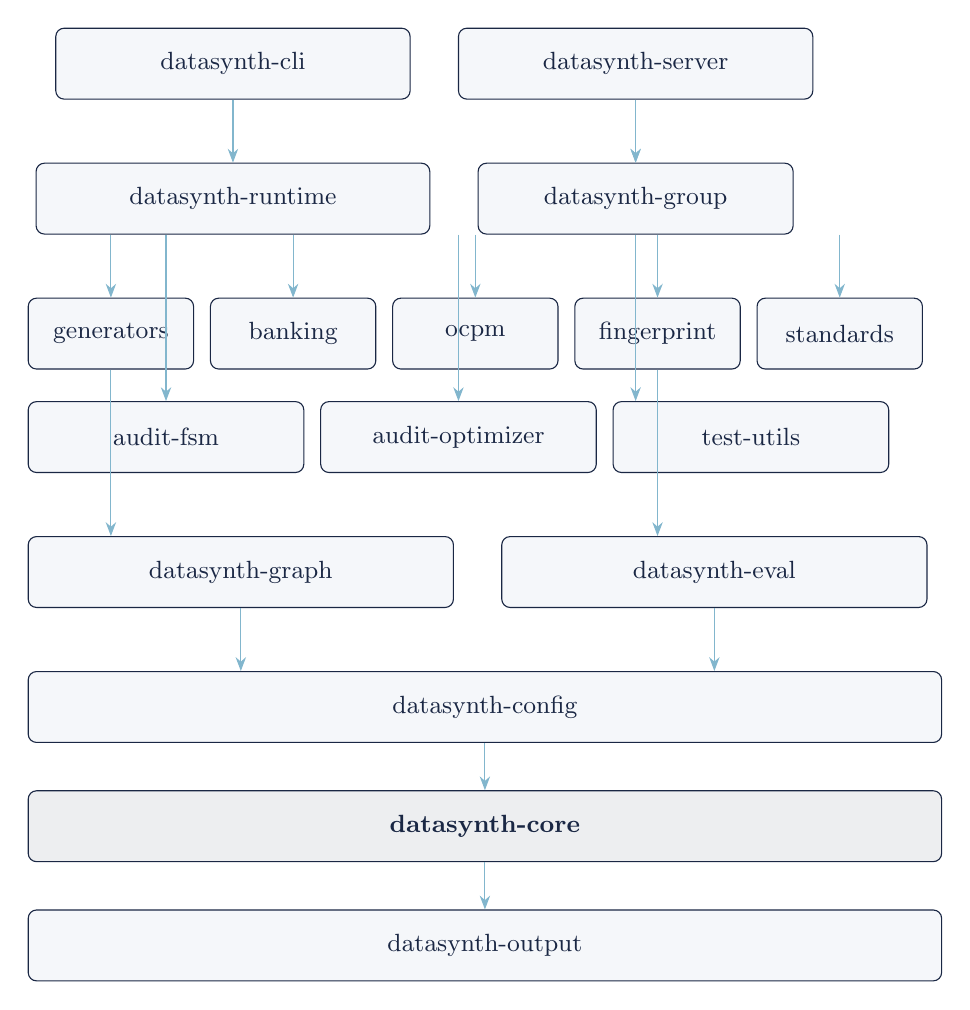
\begin{tikzpicture}[
  node distance=0.5cm,
  layer/.style={draw=brand, fill=lightbg, rounded corners=3pt,
                minimum height=0.9cm, font=\small, text=brand, align=center},
  arr/.style={-{Stealth[length=5pt]}, color=accent!60}
]
  % Top: entry-points
  \node[layer, minimum width=4.5cm] (cli) {datasynth-cli};
  \node[layer, minimum width=4.5cm, right=0.6cm of cli] (server) {datasynth-server};

  % Runtime + group
  \node[layer, minimum width=5.0cm, below=0.8cm of cli] (runtime) {datasynth-runtime};
  \node[layer, minimum width=4.0cm, right=0.6cm of runtime] (group) {datasynth-group};

  % Generators row 1
  \node[layer, minimum width=2.1cm, below=0.8cm of runtime.south west,
        anchor=north west, xshift=-0.1cm] (gen) {generators};
  \node[layer, minimum width=2.1cm, right=0.2cm of gen] (bank) {banking};
  \node[layer, minimum width=2.1cm, right=0.2cm of bank] (ocpm) {ocpm};
  \node[layer, minimum width=2.1cm, right=0.2cm of ocpm] (fp) {fingerprint};
  \node[layer, minimum width=2.1cm, right=0.2cm of fp] (std) {standards};

  % Generators row 2 — audit crates
  \node[layer, minimum width=3.5cm, below=0.4cm of gen.south west,
        anchor=north west] (fsm) {audit-fsm};
  \node[layer, minimum width=3.5cm, right=0.2cm of fsm] (opt) {audit-optimizer};
  \node[layer, minimum width=3.5cm, right=0.2cm of opt] (tu) {test-utils};

  % Analytics layer
  \node[layer, minimum width=5.4cm, below=0.8cm of fsm.south west,
        anchor=north west] (graph) {datasynth-graph};
  \node[layer, minimum width=5.4cm, right=0.6cm of graph] (eval) {datasynth-eval};

  % Config
  \node[layer, minimum width=11.6cm, below=0.8cm of graph.south west,
        anchor=north west] (config) {datasynth-config};

  % Core
  \node[layer, minimum width=11.6cm, below=0.6cm of config, fill=brand!8]
    (core) {\textbf{datasynth-core}};

  % Output
  \node[layer, minimum width=11.6cm, below=0.6cm of core] (output) {datasynth-output};

  % Arrows -- top to runtime
  \draw[arr] (cli.south) -- (runtime.north);
  \draw[arr] (server.south) -- (server.south |- runtime.north);
  \draw[arr] (cli.south -| group.north) -- (group.north);

  % Runtime to generators
  \draw[arr] (runtime.south -| gen) -- (gen.north);
  \draw[arr] (runtime.south -| bank) -- (bank.north);
  \draw[arr] (runtime.south -| ocpm) -- (ocpm.north);
  \draw[arr] (runtime.south -| fp) -- (fp.north);
  \draw[arr] (runtime.south -| std) -- (std.north);
  \draw[arr] (runtime.south -| fsm) -- (fsm.north);
  \draw[arr] (runtime.south -| opt) -- (opt.north);
  \draw[arr] (group.south) -- (group.south |- tu.north);

  % Generators to analytics
  \draw[arr] (gen.south) -- (gen.south |- graph.north);
  \draw[arr] (fp.south) -- (fp.south |- eval.north);

  % Analytics to config
  \draw[arr] (graph.south) -- (graph.south |- config.north);
  \draw[arr] (eval.south) -- (eval.south |- config.north);

  \draw[arr] (config.south) -- (core.north);
  \draw[arr] (core.south) -- (output.north);
\end{tikzpicture}
\end{center}

\subsection{Crate Roles}

\renewcommand{\arraystretch}{1.2}
\begin{tabularx}{\textwidth}{@{}>{\bfseries\color{brand}}l X@{}}
\toprule
\textbf{Crate} & \textbf{Role} \\
\midrule
\texttt{datasynth-cli}             & Binary --- generate, validate, init, info, fingerprint, templates, group, scenario, optimizer \\
\texttt{datasynth-server}          & REST + gRPC + WebSocket server with API-key + JWT auth, RBAC, rate limiting \\
\texttt{datasynth-runtime}         & EnhancedOrchestrator coordinating $\sim$30 generation phases \\
\texttt{datasynth-group}           & Multi-entity manifest / shard / aggregate engine (v5.0+) \\
\texttt{datasynth-generators}      & Domain generators (JE, document flows, subledgers, anomalies, audit) \\
\texttt{datasynth-banking}         & KYC / AML banking with fraud typologies \\
\texttt{datasynth-ocpm}            & OCEL 2.0 process mining \\
\texttt{datasynth-fingerprint}     & Privacy-preserving fingerprint extract / synthesis \\
\texttt{datasynth-standards}       & Accounting / audit standards (IFRS, US GAAP, French GAAP, German GAAP, ISA, SOX, PCAOB) \\
\texttt{datasynth-graph}           & Graph export (PyTorch Geometric, Neo4j, DGL, RustGraph) \\
\texttt{datasynth-eval}            & Evaluation framework with auto-tuning \\
\texttt{datasynth-config}          & Configuration schema, validation, presets \\
\texttt{datasynth-core}            & Domain models, traits, distributions, resource guards, templates \\
\texttt{datasynth-output}          & Output sinks (CSV, JSON, NDJSON, Parquet, XBRL, FEC, GoBD, SAP, Oracle, NetSuite) \\
\texttt{datasynth-test-utils}      & Test fixtures \\
\texttt{datasynth-audit-fsm}       & Typed audit-methodology layer (v5.5.0): Big-4 spine, jurisdictional overlays, KYC, banking forms, RMM, L4 graph, Merkle \\
\texttt{datasynth-audit-optimizer} & Risk-scoping / portfolio / Monte-Carlo / conformance analytics \\
\bottomrule
\end{tabularx}

\subsection{Production-Grade Infrastructure}

\renewcommand{\arraystretch}{1.2}
\begin{tabularx}{\textwidth}{@{}>{\bfseries\color{brand}}l X@{}}
\toprule
\textbf{Capability} & \textbf{Details} \\
\midrule
Deterministic Output & ChaCha8 PRNG with configurable seed; identical seed $\Rightarrow$ identical dataset. \\
Financial Precision  & \texttt{rust\_decimal} throughout; no IEEE 754 floating-point artefacts; decimals serialised as strings. \\
Resource Guards      & Unified CPU, memory, and disk monitoring with automatic throttling and graceful degradation (Normal\,$\to$\,Reduced\,$\to$\,Minimal\,$\to$\,Emergency). \\
Collision-Free IDs   & FNV-1a hash-based UUID factory with generator-type discriminators prevents document-ID collisions across parallel generators. UUID v5 for stable per-line transaction IDs. \\
Streaming Output     & CSV, JSON, NDJSON, Apache Parquet (Zstd compression), and XBRL 2.1 instances (US GAAP \& IFRS taxonomies). Streaming sinks with backpressure (Block, DropOldest, DropNewest, Buffer). \\
API Layer            & REST + gRPC + WebSocket with Argon2id API-key auth, JWT/OIDC bearer tokens (RS256, Keycloak / Auth0 / Entra ID), RBAC (Admin / Operator / Viewer), sliding-window rate limiting (in-memory or Redis), TLS via rustls. \\
Plugin SDK           & \texttt{GeneratorPlugin}, \texttt{SinkPlugin}, \texttt{TransformPlugin} traits with thread-safe registry. \\
Webhooks             & Fire-and-forget event dispatch (RunStarted / Completed / Failed / GateViolation) with HMAC signing and configurable retry. \\
Data Lineage         & Per-file SHA-256 checksums, \texttt{LineageGraph} tracking config $\to$ generator $\to$ output relationships, W3C PROV-JSON export, CLI \texttt{verify}. \\
COA Coverage Invariant & Always-on test asserting every generated JE \texttt{gl\_account} exists in the chart of accounts; strict-mode CLI flag fails the run on orphans. \\
\bottomrule
\end{tabularx}

% ══════════════════════════════════════════════════════════════════════════════
\newpage
\section{Compliance \& Governance}

\subsection{EU AI Act Posture}

DataSynth is a synthetic-data generator, not a high-risk AI system: outputs
are synthesised data points, not decisions about natural persons. The
platform nonetheless ships features useful for compliant downstream use:

\begin{itemize}[leftmargin=1.2em, itemsep=3pt]
  \item Generator name, version, timestamp, seed, and config hash
        machine-readable in every output run.
  \item Per-file SHA-256 checksums and W3C PROV-JSON lineage for
        reproducibility audits.
  \item Differential-privacy budgets emitted as machine-readable
        certificates when fingerprinting is used.
  \item Ground-truth labels (fraud, anomaly, data-quality issue,
        ISA 240 manual flag) for fairness and bias evaluation of
        downstream models.
\end{itemize}

\subsection{Regulatory Compliance Documentation}

Generated audit artefacts include the metadata required by the relevant
standard frameworks (ISA / PCAOB / SOX / SOC 2 / CSRD), with cross-reference
tables and jurisdiction profiles for cross-border engagements. Working-paper
bundles are SHA-256 Merkle-rooted with replay-protected inclusion proofs
(ISA 230 working-paper management).

\subsection{Quality Gates}

Three quality-gate profiles --- \texttt{lenient}, \texttt{default},
\texttt{strict} --- combine balance-equation, distribution-fit, copula-recovery,
Benford-MAD, completeness, and coherence checks. The auto-tune loop and the
CI pipeline both consume the same gate definitions.

% ══════════════════════════════════════════════════════════════════════════════
\newpage
\section{Getting Started}

\subsection{Quick Start (Single Entity)}

\begin{tcolorbox}[notebox={CLI}]
\small
\begin{verbatim}
git clone https://github.com/mivertowski/SyntheticData.git && cd SyntheticData
cargo build --release

# Demo --- generates a complete dataset with defaults
./target/release/datasynth-data generate --demo --output ./output

# Initialise + generate from a config
./target/release/datasynth-data init --industry manufacturing \
                                     --complexity medium \
                                     -o config.yaml
./target/release/datasynth-data validate --config config.yaml
./target/release/datasynth-data generate --config config.yaml \
                                         --output ./output \
                                         --validate-coa-coverage
\end{verbatim}
\end{tcolorbox}

\subsection{Group Audit Pipeline}

\begin{tcolorbox}[notebox={Multi-entity consolidation}]
\small
\begin{verbatim}
# Single-period
datasynth-data group generate \
  --config configs/examples/group/mini_nestle.yaml \
  --out ./group_archive

# Multi-period (chained continuity)
datasynth-data group generate-chain \
  --config configs/examples/group/mini_nestle.yaml \
  --periods 4 \
  --out ./group_archive_q1_q4

# Or use the explicit three-phase pipeline
datasynth-data group manifest    --config group.yaml --out manifest.json
datasynth-data group shard       --manifest manifest.json --shard-id S_SIG_0001 \
                                 --out ./shards/S_SIG_0001/
datasynth-data group aggregate   --manifest manifest.json --shards-dir ./shards \
                                 --out ./group_archive
\end{verbatim}
\end{tcolorbox}

\subsection{Fingerprint-Driven Synthesis}

\begin{tcolorbox}[notebox={From real data to defensible synthetic}]
\small
\begin{verbatim}
# 1. Extract a privacy-preserving fingerprint from real data
datasynth-data fingerprint extract \
  --input  ./real_journals.csv \
  --output ./real.dsf \
  --privacy-level standard

# 2. Validate the .dsf file
datasynth-data fingerprint validate ./real.dsf

# 3. Generate matched synthetic data
datasynth-data generate --fingerprint ./real.dsf \
                        --scale 1.0 \
                        --output ./synthetic

# 4. Evaluate fidelity
datasynth-data fingerprint evaluate \
  --fingerprint ./real.dsf \
  --synthetic   ./synthetic/
\end{verbatim}
\end{tcolorbox}

\subsection{Server Mode}

\begin{tcolorbox}[notebox={REST / gRPC / WebSocket}]
\small
\begin{verbatim}
cargo run -p datasynth-server -- --port 3000 --worker-threads 4

# REST: /api/config, /api/stream/{start|stop|pause|resume},
#       /api/stream/trigger/{pattern}
# WebSocket: /ws/events
# Auth: X-API-Key header (Argon2id) or Bearer JWT
\end{verbatim}
\end{tcolorbox}

\subsection{Python Integration}

The open-source \texttt{datasynth-py} wrapper has been retired (v4.4.3).
Recommended paths:

\begin{itemize}[leftmargin=1.2em, itemsep=3pt]
  \item \textbf{Commercial SDKs} --- official typed Python and TypeScript
        SDKs at \href{https://vynfi.com}{vynfi.com}.
  \item \textbf{Subprocess + dataframes} --- invoke the \texttt{datasynth-data}
        CLI from Python via \texttt{subprocess} and read the generated
        CSV / JSON / Parquet outputs with \texttt{pandas} / \texttt{polars}
        / \texttt{pyarrow}.
  \item \textbf{HuggingFace} --- skip generation and pull a pre-built
        reference dataset from \href{https://huggingface.co/VynFi}{huggingface.co/VynFi}.
\end{itemize}

\subsection{Companion Academic Paper}

The formal treatment of distributional properties, copula construction,
DP composition, and the reference-knowledge-graph framework appears in:

\begin{tcolorbox}[notebox={Citation}]
\small
Ivertowski, M.\ (2026).
\textit{DataSynth: Reference Knowledge Graphs for Enterprise Audit Analytics
through Synthetic Data Generation with Provable Statistical Properties.}
SSRN Working Paper. \url{\dsssrnurl}
\\[2pt]
In-repo source: \texttt{paper/main.tex}.
\end{tcolorbox}

% ══════════════════════════════════════════════════════════════════════════════
\bibliographystyle{plainnat}
\bibliography{references}

% ══════════════════════════════════════════════════════════════════════════════
\vspace*{\fill}
\begin{center}
\rule{0.5\textwidth}{0.4pt}\\[0.6em]
\textcolor{midgray}{\small
  DataSynth v\dsversion{} \textbullet{}
  \dsdate{} \textbullet{}
  \href{\dsrepourl}{GitHub}
  \textbullet{}
  Apache-2.0
}
\end{center}

\end{document}
